\documentclass[aspectratio=169, 11pt]{beamer}

% ── Theme & Colors ──────────────────────────────────────────
\usetheme{Madrid}
\usecolortheme{default}

\definecolor{darkcharcoal}{HTML}{2C3E50}
\definecolor{accentblue}{HTML}{2980B9}
\definecolor{donegreen}{HTML}{27AE60}
\definecolor{pendinggray}{HTML}{BDC3C7}
\definecolor{lightbg}{HTML}{F8F9FA}
\definecolor{darktext}{HTML}{1A1A2E}

\setbeamercolor{structure}{fg=darkcharcoal}
\setbeamercolor{palette primary}{bg=darkcharcoal, fg=white}
\setbeamercolor{palette secondary}{bg=accentblue, fg=white}
\setbeamercolor{frametitle}{bg=darkcharcoal, fg=white}
\setbeamercolor{title}{fg=darkcharcoal}
\setbeamercolor{subtitle}{fg=accentblue}
\setbeamercolor{block title}{bg=darkcharcoal, fg=white}
\setbeamercolor{block body}{bg=lightbg, fg=darktext}
\setbeamercolor{item}{fg=accentblue}

\setbeamertemplate{navigation symbols}{}
\setbeamerfont{frametitle}{size=\large, series=\bfseries}
\setbeamerfont{title}{size=\Large, series=\bfseries}

% ── Packages ────────────────────────────────────────────────
\usepackage{tikz}
\usetikzlibrary{shapes.geometric, arrows.meta, positioning, fit, calc}
\usepackage{amsmath, amssymb}
\usepackage{booktabs}
\usepackage{graphicx}
\usepackage{hyperref}
\usepackage{xcolor}
\usepackage{array}

% ── TikZ Styles ─────────────────────────────────────────────
\tikzstyle{block} = [rectangle, rounded corners, minimum width=2.2cm, minimum height=0.8cm, text centered, draw=darkcharcoal, fill=lightbg, font=\small]
\tikzstyle{done} = [block, draw=donegreen, fill=donegreen!10, text=donegreen!80!black]
\tikzstyle{pending} = [block, draw=pendinggray, fill=pendinggray!15, text=pendinggray!60!black]
\tikzstyle{arrow} = [-{Stealth[length=2.5mm]}, thick, color=darkcharcoal!70]

% ── Meta ────────────────────────────────────────────────────
\title{Optimising Fed-Batch Bioprocesses using pyFOOMB}
\subtitle{UG Project Progress Report}
\author{Yashashwi Singhania }
% \institute{Department of Biochemical Engineering\\Indian Institute of Technology (BHU), Varanasi}
\date{November 2026}

% ═══════════════════════════════════════════════════════════
\begin{document}

% ── Slide 1: Title ──────────────────────────────────────────
\begin{frame}[plain]
  \vfill
  \begin{center}
    
\includegraphics[height=1.55cm]{iit_bhu_logo.png}\\[0.5cm]
    {\Large\bfseries\color{darkcharcoal} Indian Institute of Technology (BHU), Varanasi}\\[0.6cm]
    {\LARGE\bfseries\color{darkcharcoal} Optimising Fed-Batch Bioprocesses}\\[0.15cm]
    {\LARGE\bfseries\color{darkcharcoal} using pyFOOMB}\\[0.4cm]
    {\large\color{accentblue} UG Project Report -- Semester VII}\\[0.8cm]
    \begin{tabular}{rl}
      \textbf{Student:} & Yashashwi Singhania (23014019) \\
      \textbf{Guide:} & Dr.\ Sharon Mano Pappu J. \\
      \textbf{Department:} & Biochemical Engineering \\
      \textbf{Lab:} & Bioprocess Development and Digitalization Laboratory \\
    \end{tabular}\\[0.5cm]
    {\small November 2026}
  \end{center}
  \vfill
\end{frame}

\begin{frame}{From Growth Kinetics to Feed Design}
  \begin{block}{Question I carried forward}
    How should I feed a growing culture to maximise the amount of product at harvest?
  \end{block}
  \begin{itemize}
    \item In Semester VI, I fitted the specific production rate $q_p$ as a function of growth rate $\mu$ for nine literature cases.
    \item This semester, I used those fits in pyFOOMB to compare feed schedules over a full batch and fed-batch simulation.
    \item I then tested whether allowing the pump to change its feeding law mid-run improved the best result.
  \end{itemize}
\end{frame}

\begin{frame}{Batch and Fed-Batch Simulation}
  \begin{block}{Batch}
    I let the cells grow on the initial substrate with the pump off. At the substrate threshold, the simulated biomass, substrate, product and volume carry into fed-batch.
  \end{block}
  \begin{block}{Fed-batch}
    I simulate each candidate feed over 40 hours. The pump stops at 4 L and the culture continues to the end of the simulation.
  \end{block}
  \[
      F(t)\longrightarrow S(t)\longrightarrow \mu(t)
      \longrightarrow q_p(\mu)\longrightarrow P(t)V(t).
  \]
  \small These comparisons used a common 1 L starting volume, 20 g/L substrate and a 0.5 g/L feed-start threshold.
\end{frame}

\begin{frame}{How I Optimised the Feed}
  \begin{itemize}
    \item For each product and feed family, I searched over the pump settings with differential evolution.
    \item Each candidate was scored on total product at harvest, $P(t_f)V(t_f)$.
    \item I replayed candidate settings with tighter CVode tolerances and checked the working-volume limit.
    \item I expanded seven feed families to eleven, giving 99 product--strategy combinations across nine datasets.
  \end{itemize}
\end{frame}

\begin{frame}{Two-Stage Feed Schedules}
  \centering
  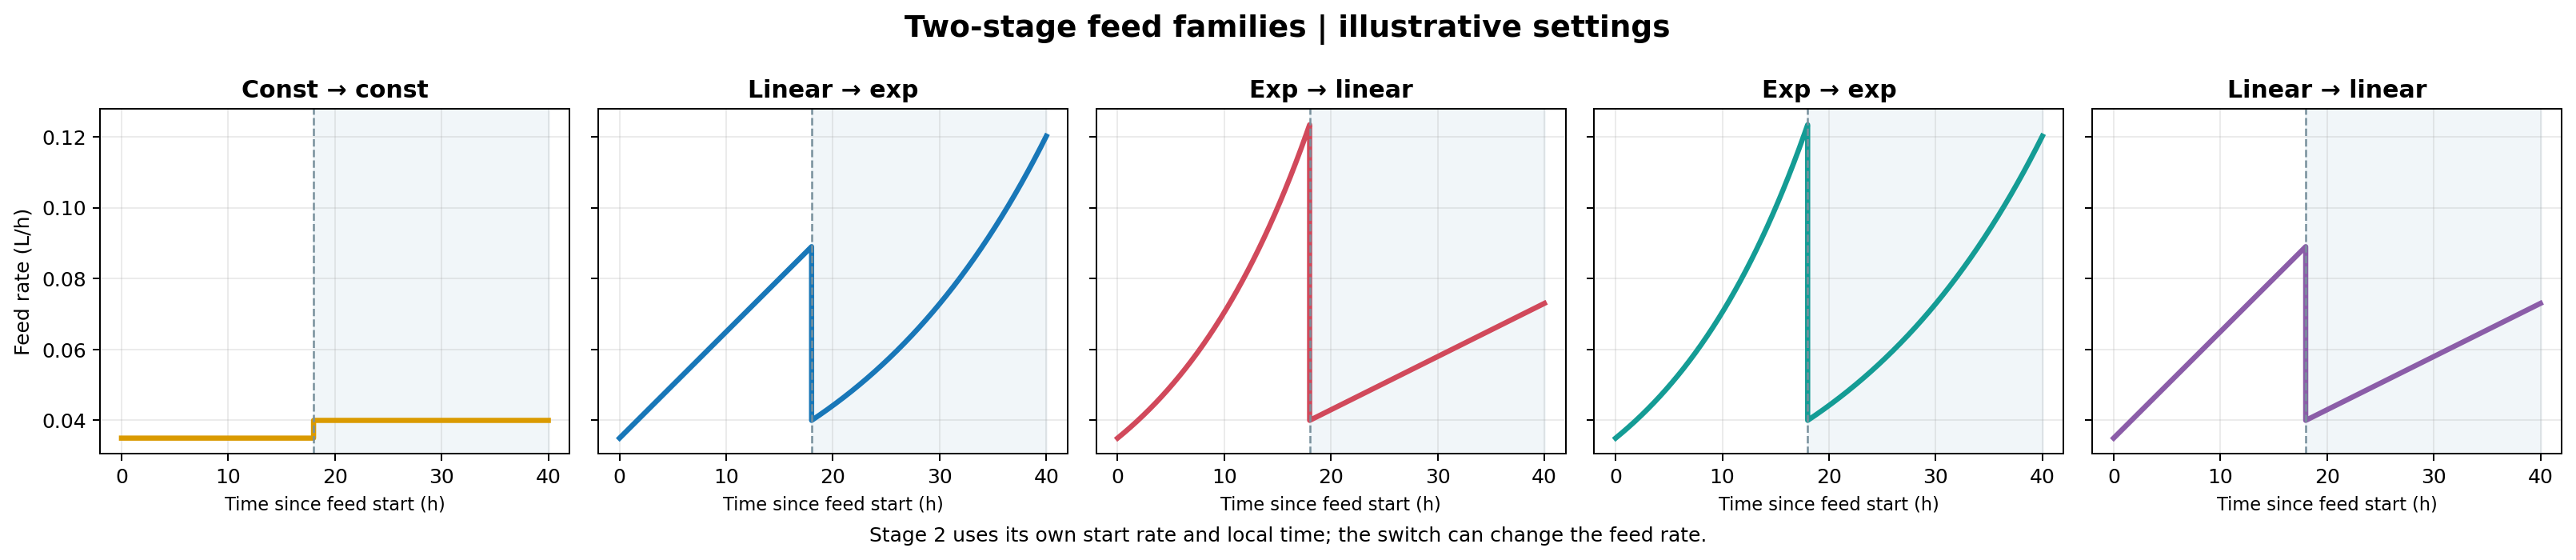
\includegraphics[width=\linewidth]{pyfoomb_results/two_stage_extension/final/two_stage_schematics.png}
  \begin{block}{What I varied}
    I searched for the switch time and the starting rate and slope or exponent of each stage. Stage two has its own clock and can begin at a different pump rate.
  \end{block}
\end{frame}

\begin{frame}{Total Product Across Eleven Strategies}
  \centering
  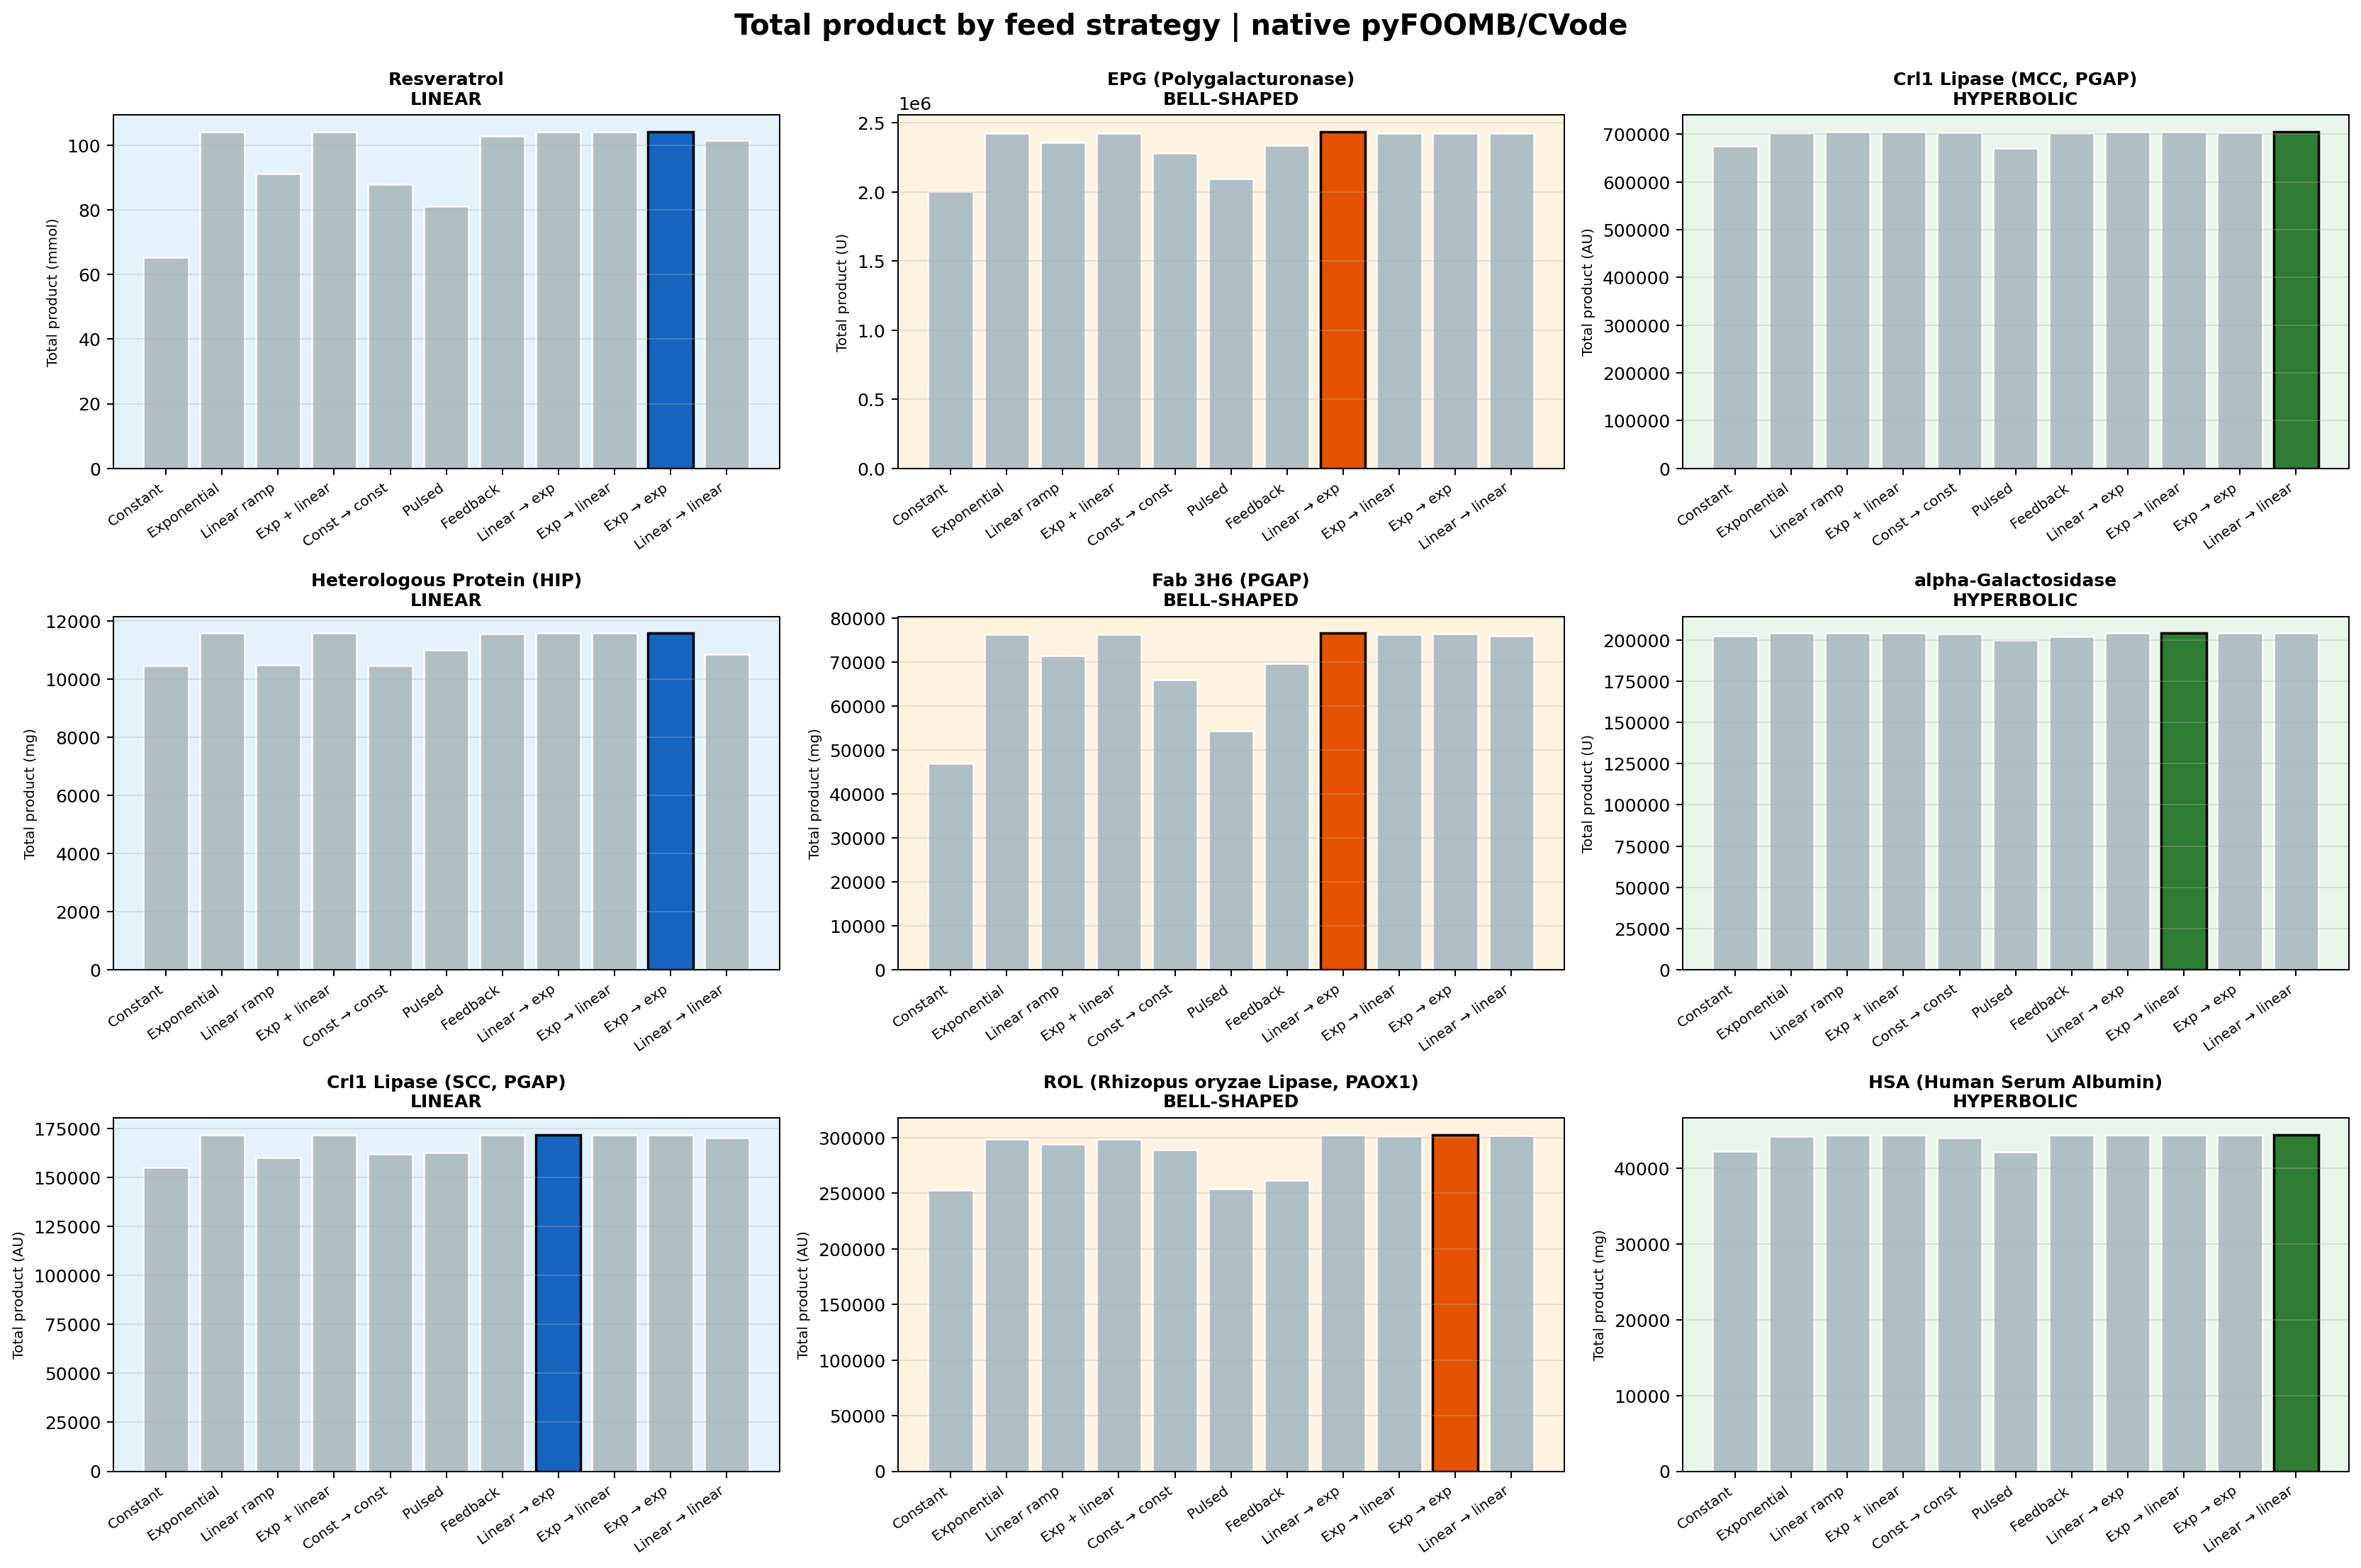
\includegraphics[width=\linewidth,height=.80\textheight,keepaspectratio]{pyfoomb_results/two_stage_extension/final/strategy_comparison.png}
\end{frame}

\begin{frame}{What Changed After Adding a Second Stage?}
  \centering
  \begin{tabular}{lll}
    \toprule
    Product & Best schedule found & Gain over earlier best \\
    \midrule
    ROL lipase & Exponential $\to$ exponential & $+1.28\%$ \\
    EPG & Linear $\to$ exponential & $+0.49\%$ \\
    Fab case in current model & Linear $\to$ exponential & $+0.40\%$ \\
    Crl1 lipase (MCC) & Linear $\to$ linear & $+0.10\%$ \\
    \bottomrule
  \end{tabular}
  \vspace{.35cm}
  \begin{block}{What I found}
    The extra stage gave ROL the largest improvement. Five datasets gained less than $0.01\%$ under the common simulation settings.
  \end{block}
\end{frame}

\begin{frame}{Biomass, Substrate and Product Profiles}
  \centering
  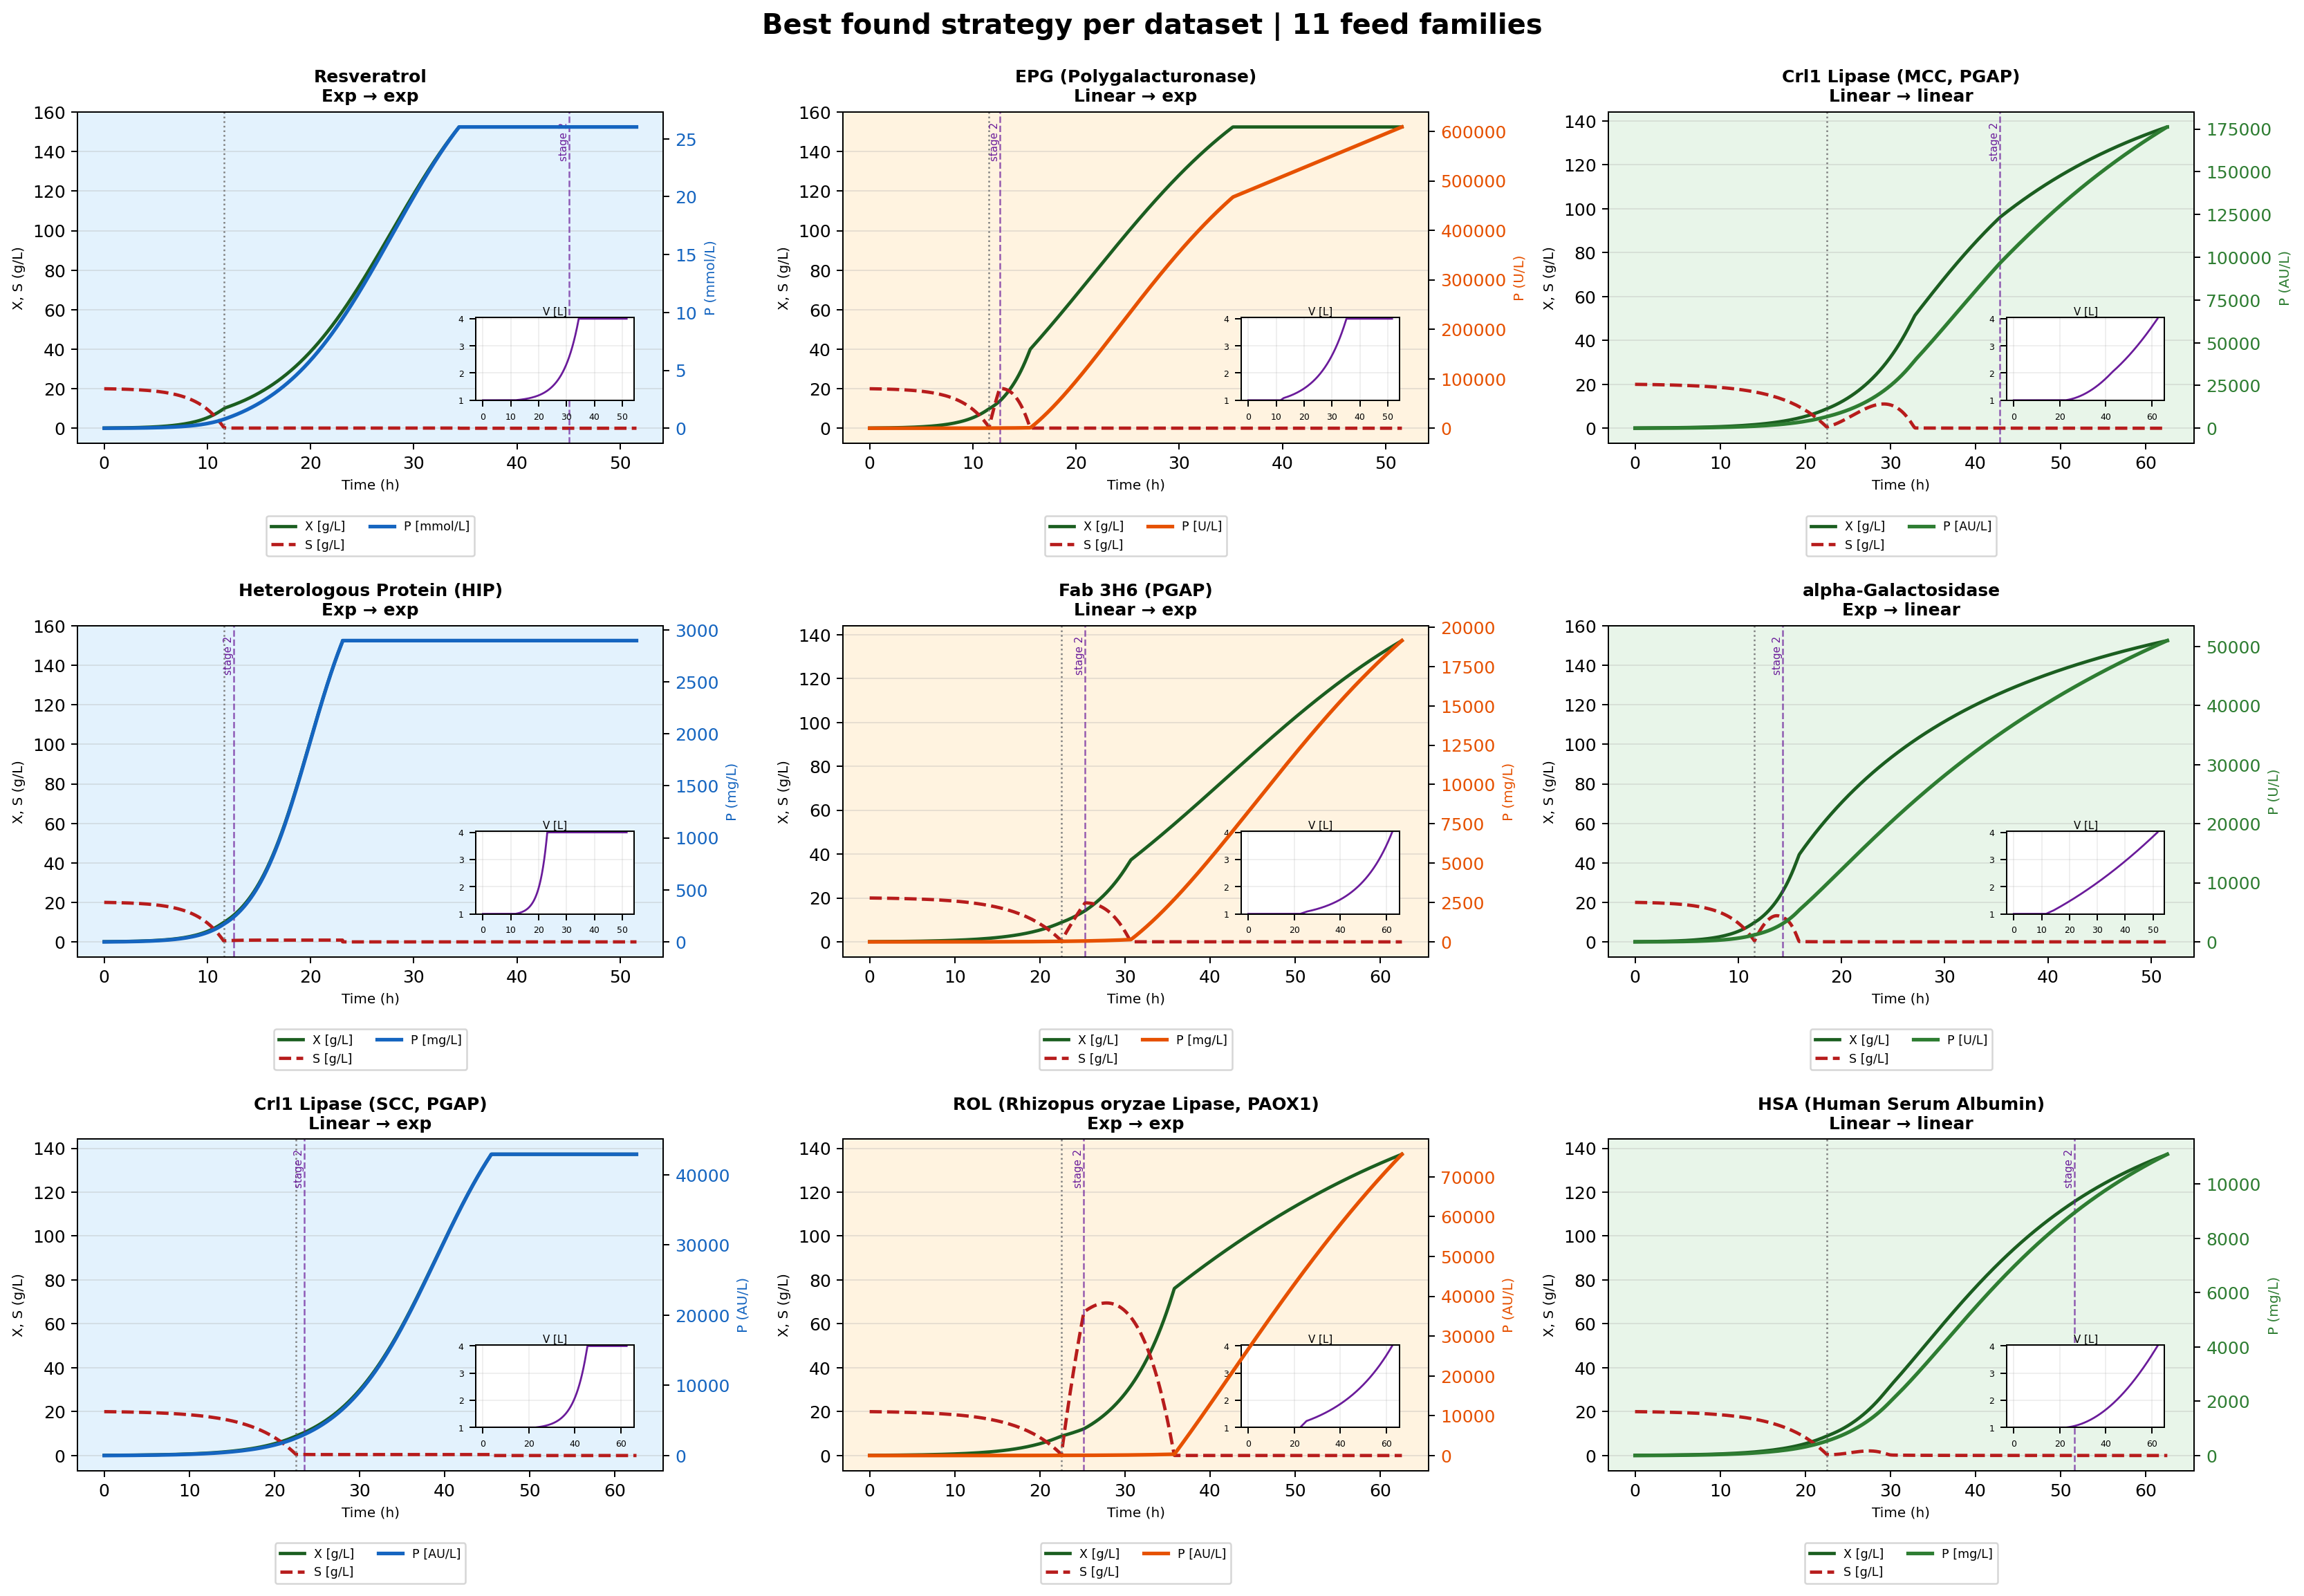
\includegraphics[width=\linewidth,height=.80\textheight,keepaspectratio]{pyfoomb_results/two_stage_extension/final/best_profiles.png}
\end{frame}

\begin{frame}{Actual Pump Rates During Fed-Batch}
  \centering
  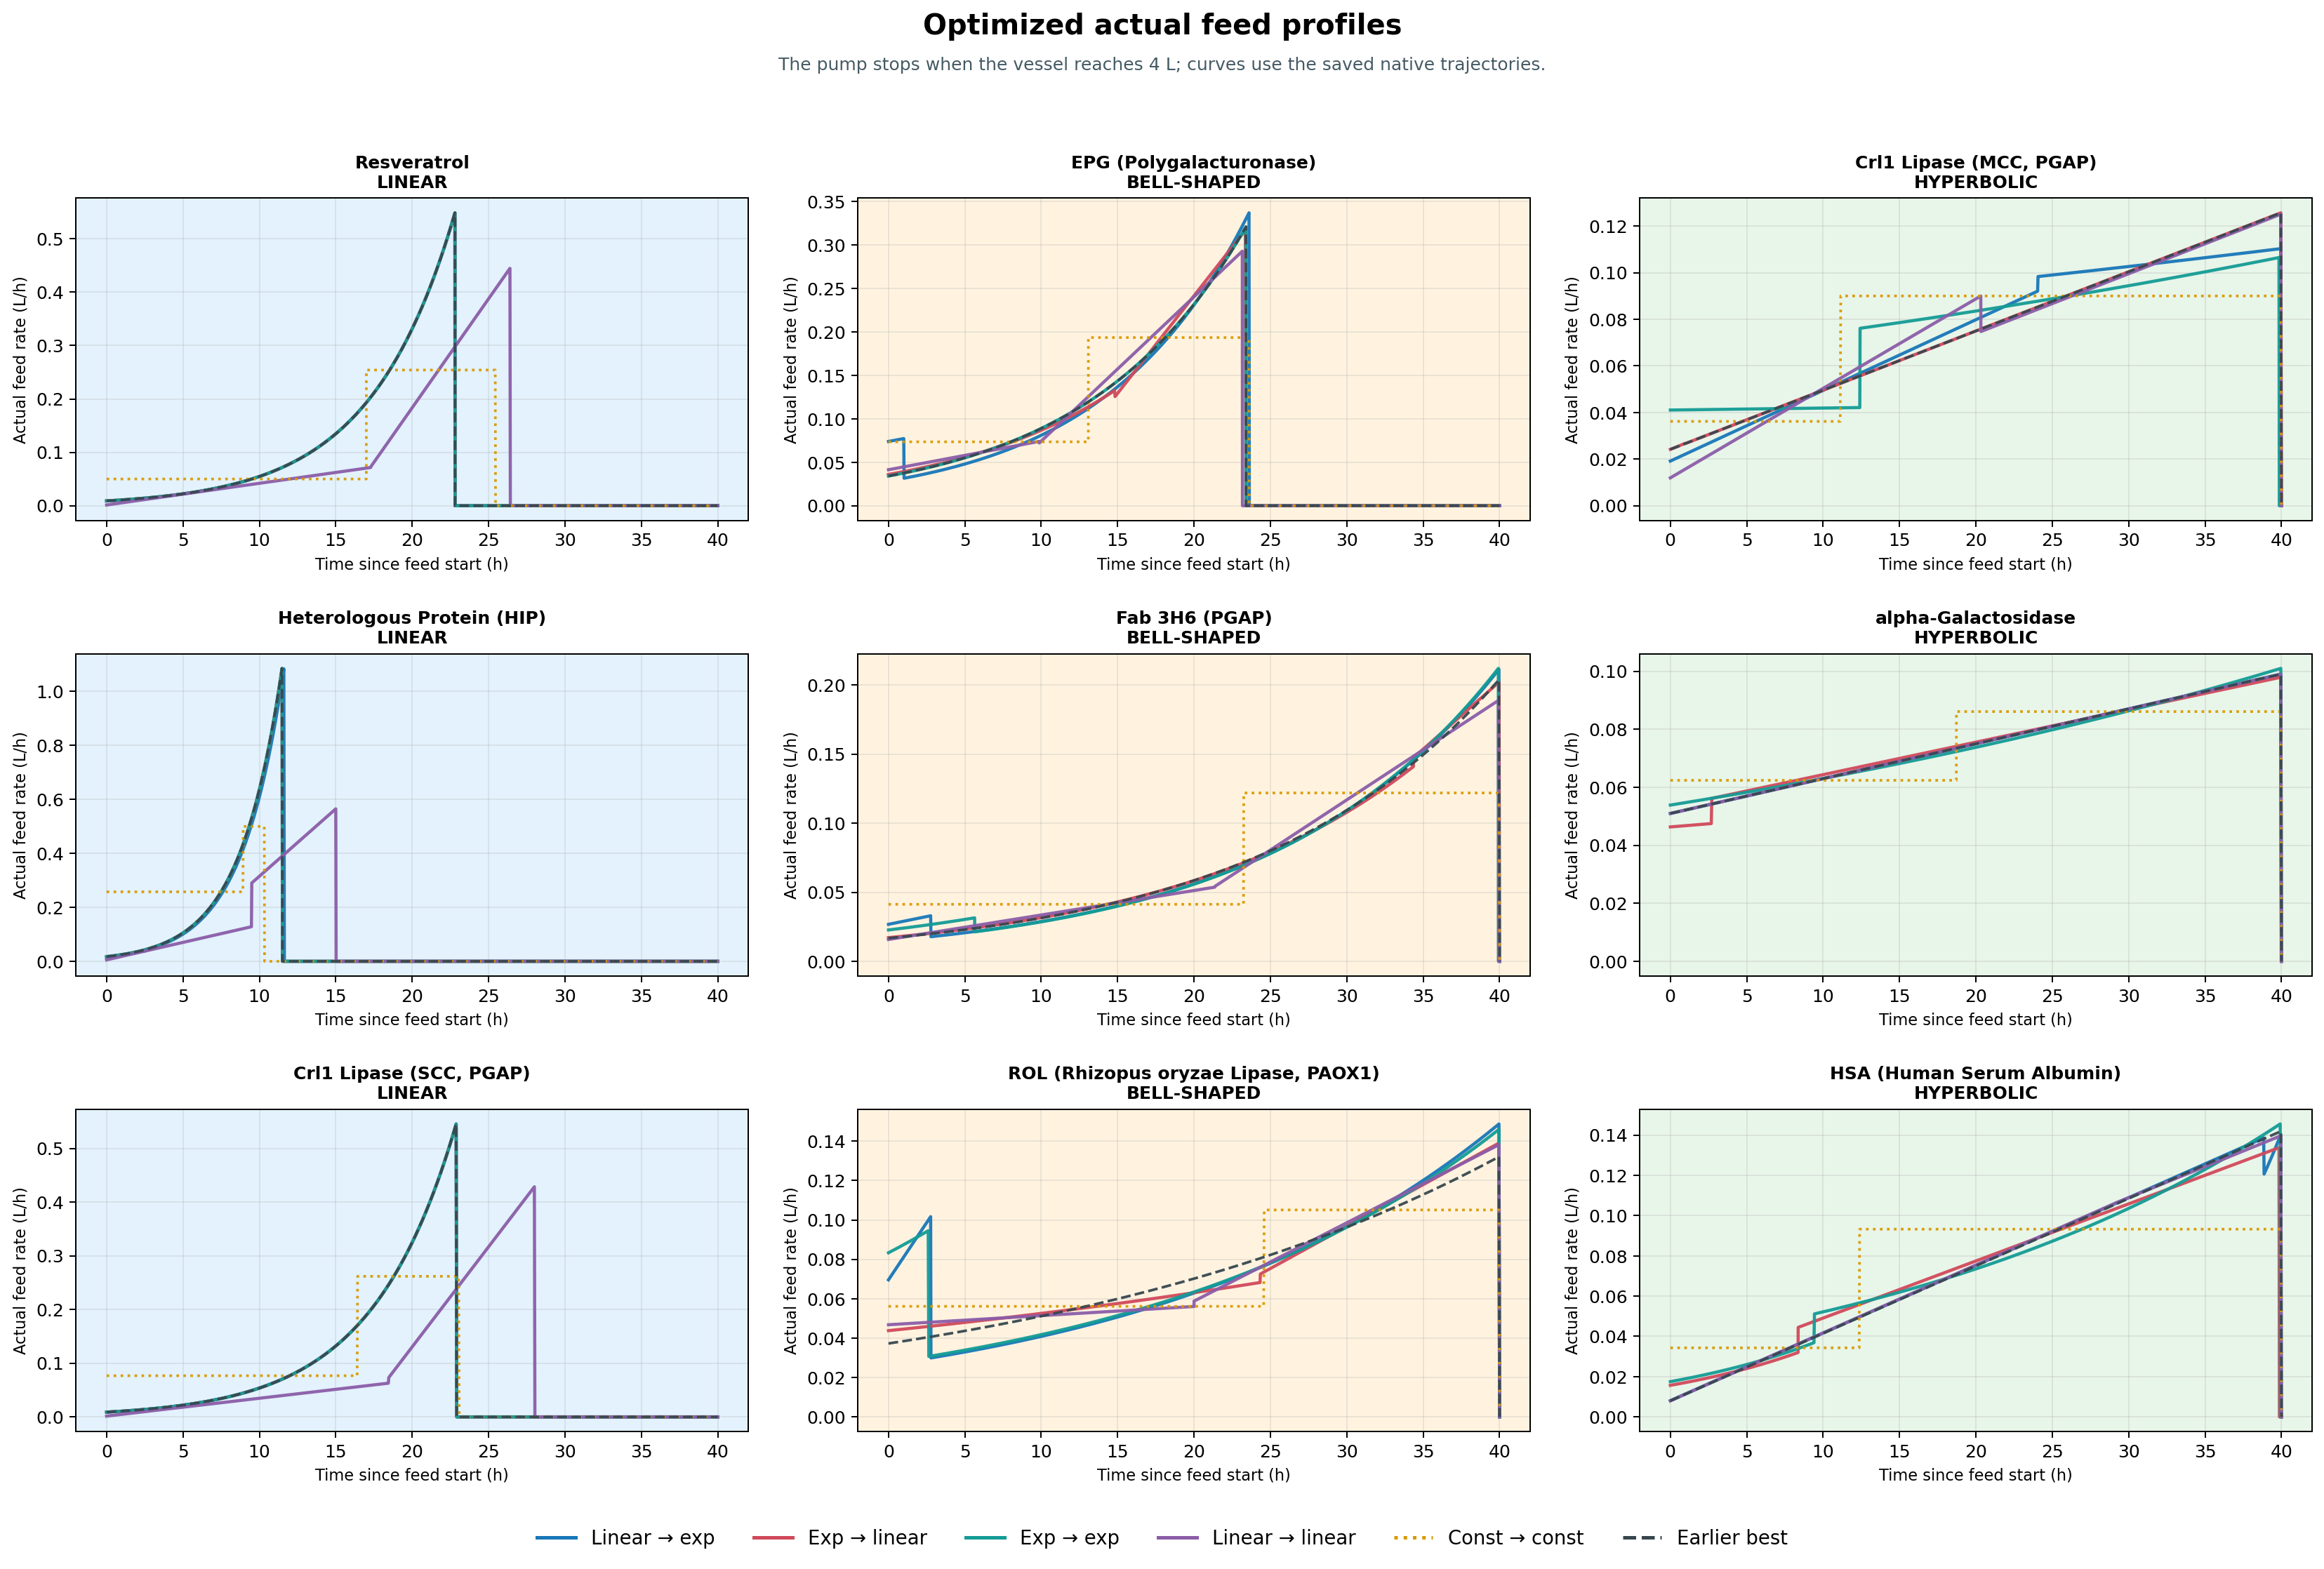
\includegraphics[width=\linewidth,height=.80\textheight,keepaspectratio]{pyfoomb_results/two_stage_extension/final/two_stage_feed_profiles.png}
\end{frame}

\begin{frame}{Benchmarking Against the Original Experiment}
  \begin{block}{Fab 2F5 case from Garc\'ia-Ortega et al. (2013)}
    The experiment began with 2 L and 40 g/L glycerol. At glycerol depletion the authors began an exponential glucose feed. Figure 2A reports biomass, substrate and Fab concentrations for a nominal growth rate of $0.10\,\mathrm{h}^{-1}$.
  \end{block}
  \begin{itemize}
    \item I identified this run as a benchmark for the batch-to-feed transition and product trajectory.
    \item My next comparison is to replay the published conditions and overlay the model and experimental curves. For each other case, I need to identify the matching experiment and record its conditions and stopping rule.
  \end{itemize}
  \footnotesize Biochemical Engineering Journal 79, 172--181. \href{https://doi.org/10.1016/j.bej.2013.07.013}{doi:10.1016/j.bej.2013.07.013}
\end{frame}

\begin{frame}[plain]
  \centering\vfill
  {\LARGE\bfseries\color{darkcharcoal} Thank you}\par\medskip
  Yashashwi Singhania
  \vfill
\end{frame}
\end{document}
